% Figure Q3, generated by experiments/q3_margin_identification.py.
\begin{figure}[t]
  \centering
  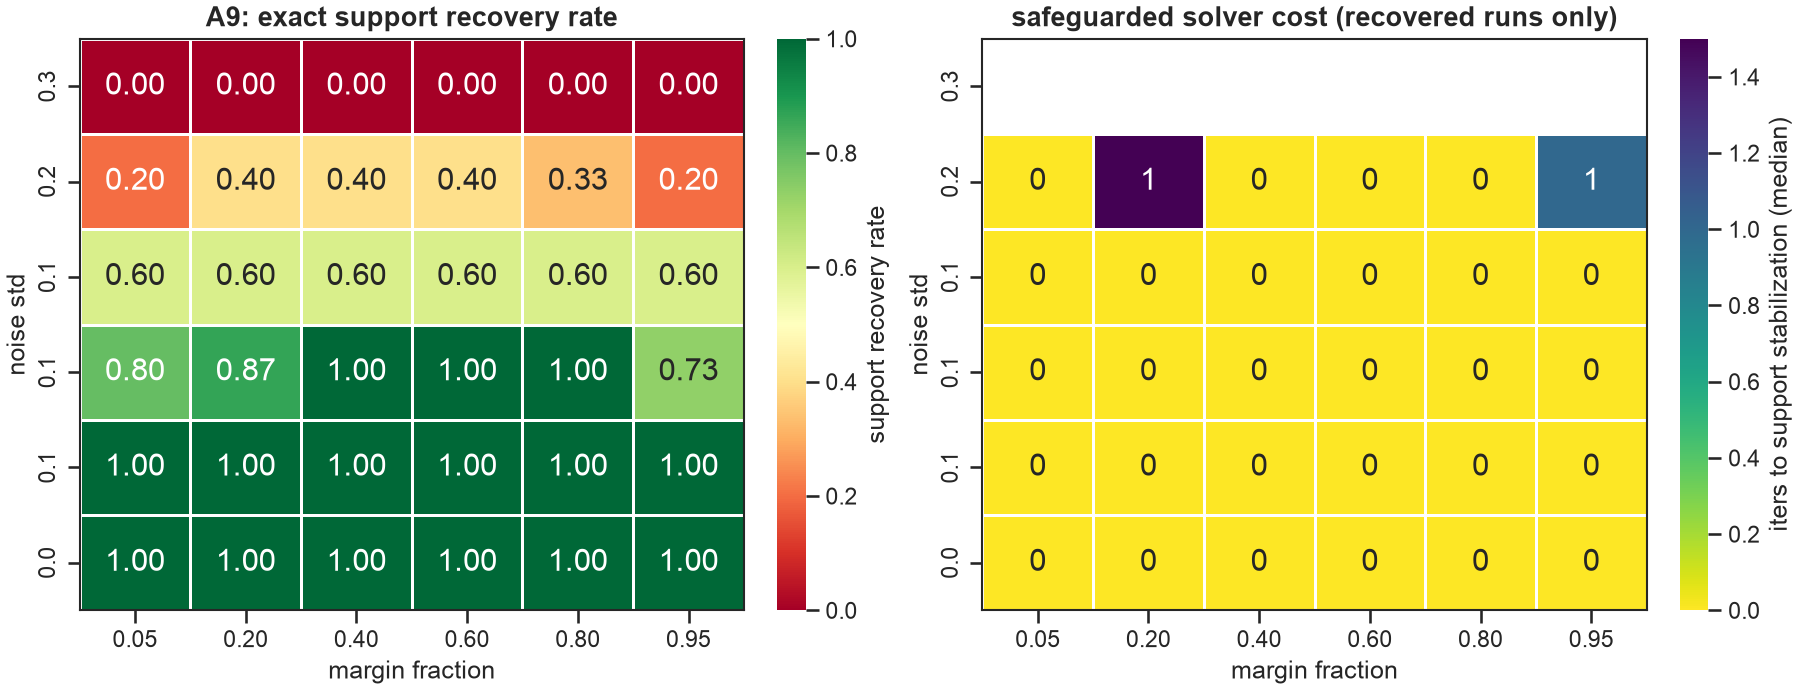
\includegraphics[width=\linewidth]{../shared/figures/generated/q3_margin_identification.png}
  \caption{\textbf{Q3, identification phase transition over (noise, margin fraction).} Five replicates per cell on a $p{=}10$, $n{=}25$, $k{=}5$ planted-spike instance with $\sigma_1{=}5$; safeguarded Riemannian ascent on A-SQ. \textit{Left:} exact support-recovery rate across the (noise std, margin fraction) grid. Recovery is uniform at $\sigma_{\mathrm{noise}}{\le}0.05$, degrades to ${\sim}0.6$ at $0.15$, and collapses by $0.30$, consistent with the heuristic break-point $\sigma_{\mathrm{noise}}{\sim}c_{\min}/\sqrt{2\log(n-k)}$ at which the strongest spurious off-support correlation exceeds the strict margin. \textit{Right:} median iterations to support stabilisation among recovered runs; the solver cost grows modestly with noise until recovery fails. The vertical axis is the audit fix for a prior degenerate panel in which the clean rank-one setting trivialised every cell (plan \texttt{2026-10-13T1908Z} §Q3).}
  \label{fig:q3-margin}
\end{figure}
